\documentclass[10pt]{article}
\usepackage[margin=0.9in]{geometry}
\usepackage{amsmath}
\usepackage{booktabs}
\usepackage{graphicx}
\usepackage{float}
\usepackage{tabularx}
\usepackage[hidelinks]{hyperref}
\usepackage{enumitem}
\usepackage{caption}
\setlist{nosep,leftmargin=*}
\captionsetup{font=small,labelfont=bf,skip=5pt}
\newcolumntype{L}{>{\raggedright\arraybackslash}X}
\renewcommand{\arraystretch}{1.15}

\title{Small-Model Alignment: SFT and DPO on Qwen2.5-0.5B}
\author{Muhammad Ahmed}
\date{}

\begin{document}
\sloppy
\maketitle

\section{Repository, Models, and Data}

\textbf{Repository:} \url{https://github.com/ahmedamirkol01-art/small-model-alignment}.
The central math is encapsulated by the file \texttt{submission\_adapter.py}, and implemented in \texttt{alignment/sft.py} and \texttt{alignment/dpo.py}.
The training, generation and judging scripts are located in the \texttt{scripts/} directory and the Kaggle notebooks are found in the \texttt{notebooks/} directory and are run in order.

\textbf{Models.} The base model is \texttt{Qwen/Qwen2.5-0.5B}~\cite{qwen}. It is trained as an instruction model by SFT, and the from-scratch DPO runs start at the SFT \texttt{best} checkpoint. The LoRA Persona run is performed using \texttt{HuggingFaceTB/SmolLM2-360M-Instruct}.

\textbf{Prompt format.} In the training and generation, the base model, SFT model and both DPO models of Qwen use the same hand-written ChatML template (with line breaks):
{\small
\begin{verbatim}
<|im_start|>system
You are a helpful assistant.<|im_end|>
<|im_start|>user
{instruction}<|im_end|>
<|im_start|>assistant
\end{verbatim}
}
\noindent The target should be the answer that is followed by the tokenizer EOS token (\texttt{<|endoftext|>}).
Prompt and response are tokenized individually without any special tokens, and the tokenized response is appended to the tokenized prompt.
EOS is added first, then the sequence is cut off at the context length, so if a response is cut off, the EOS sign will be missing.
SmolLM2 is using its own chat template via TRL and via \texttt{generate.py --use\_chat\_template}.

\textbf{Data.} All selection uses seed 42. For each split in the data set, the data is shuffled with \texttt{datasets.shuffle(seed=42)} and then filtered in order until the desired set size is reached. Table~\ref{tab:data} lists the number of examples in each set.
\begin{itemize}
\item \textbf{SFT} (\texttt{HuggingFaceH4/ultrachat\_200k}~\cite{ultrachat}): user turn 0 and assistant turn 1 of the conversation are used. If the complete formatted sequence (prompt, response and EOS) is contained in 512 tokens then it is kept. Thus, all training objectives end with an EOS.
\item \textbf{HH-RLHF} (\texttt{Anthropic/hh-rlhf}~\cite{hh}): only single turn pairs (one \texttt{Human:} and one \texttt{Assistant:} turn). Selected and rejected prompts should be identical, and the two responses should not be empty and should differ.
\item \textbf{UltraFeedback} (\texttt{HuggingFaceH4/ultrafeedback\_binarized}~\cite{uf}): single turn pairs with \texttt{score\_chosen > score\_rejected}.
\end{itemize}
Both of the DPO data sets drop prompts over 256 tokens. There is no length filter on responses: sequences are cut at 512 tokens.

\begin{table}[H]
\centering\small
\caption{Training data. Every count comes from the \texttt{data\_summary.json} of each run.}
\label{tab:data}
\begin{tabular}{lllrrr}
\toprule
\textbf{Track} & \textbf{Dataset} & \textbf{Splits (train / val)} & \textbf{Train} & \textbf{Val} & \textbf{Scanned} \\
\midrule
SFT & UltraChat-200k & train\_sft / test\_sft & 30{,}000 & 1{,}000 & 52{,}926 \\
HH-RLHF DPO & Anthropic HH-RLHF & train / test & 15{,}000 & 1{,}000 & 49{,}371 \\
UltraFeedback DPO & UltraFeedback binarized & train\_prefs / test\_prefs & 15{,}000 & 1{,}000 & 21{,}366 \\
LoRA persona DPO & persona preferences & random split, seed 42 & 200 & 20 & 220 \\
\bottomrule
\end{tabular}
\end{table}

\textbf{Evaluation sets.}
\begin{itemize}
\item HH-RLHF DPO: there are 10 categories of 30 prompts each, for a total of 300 prompts in the provided \texttt{eval\_sets/hh\_rlhf\_eval\_300\_seed42.json}.
\item UltraFeedback DPO: the test is based on \texttt{eval\_sets/alpaca\_eval\_300\_seed42.json}, the 300 prompt subset of \texttt{tatsu-lab/alpaca\_eval}~\cite{alpacaeval} taken with \texttt{random.Random(42).sample}.
\item LoRA: the new \texttt{eval\_sets/persona\_style\_eval.json} file is 40 new prompts, 10 in each of the four domains (cooking, coding, general help and safety-sensitive), for evaluating a model's performance in a realistic context. None of them are in the training data for the personas.
\end{itemize}

\section{Experimental Configuration}

\begin{table}[H]
\centering\small
\caption{Values used for the submitted checkpoints (from each run's \texttt{config.json}).}
\label{tab:config}
\begin{tabularx}{\textwidth}{>{\bfseries}l L L L L}
\toprule
 & \textbf{SFT} & \textbf{HH-RLHF DPO} & \textbf{UltraFeedback DPO} & \textbf{LoRA-DPO (TRL)} \\
\midrule
Init / reference & Qwen2.5-0.5B / -- & SFT best / frozen SFT best & SFT best / frozen SFT best & SmolLM2-360M-Instruct / same model, adapter off \\
Trainable params & full fine-tuning & full & full & LoRA $r{=}16$, $\alpha{=}32$, dropout 0.05 on q,k,v,o,gate,up,down \\
Optimizer & AdamW & AdamW & AdamW & AdamW (TRL default) \\
Peak LR & $2\times10^{-5}$ & $1\times10^{-6}$ & $1\times10^{-6}$ & $5\times10^{-5}$ \\
Schedule / warmup & cosine / 3\% (28 steps) & constant / none & constant / none & cosine / 10\% \\
Weight decay & 0.1 (matrices only) & 0 & 0 & 0 \\
Grad clipping & 1.0 & 1.0 & 1.0 & 1.0 \\
Batch $\times$ accum & $2\times16=32$ & $1\times32=32$ & $1\times32=32$ & $4\times2=8$ \\
Precision & fp32 weights, fp16 autocast, GradScaler & same; reference fp32 under fp16 autocast on cuda:1 & same as HH-RLHF & fp16 mixed, fp32 base \\
Max length & 512 & 512 (prompt $\le$ 256) & 512 (prompt $\le$ 256) & 512 \\
Epochs / steps & 1 / 937 & 1 / 468 & 1 / 468 & 3 / 75 \\
$\boldsymbol{\beta}$ & -- & 0.1 & 0.1 & 0.1 \\
Checkpoint & lowest val loss & best val reward acc. & best val reward acc. & final adapter \\
Seed & 42 & 42 & 42 & 42 \\
\bottomrule
\end{tabularx}
\end{table}

\textbf{Loss reduction.} SFT loss is the average of the negative log-probabilities over all the response tokens in the batch that are not masked. Labels for prompt and padding tokens contribute nothing and are equal to $-100$.
In DPO~\cite{dpo} the response-token log-probabilities of each sequence are added together to give its score.
The loss is the average over the batch of $-\log\sigma(\beta[(\log\pi_\theta(y_w|x)-\log\pi_\theta(y_l|x))-(\log\pi_{\text{ref}}(y_w|x)-\log\pi_{\text{ref}}(y_l|x))])$.
The \texttt{torch.no\_grad()} context manager is used for the reference forward pass.

\textbf{Generation.} All models are configured as follows: the temperature and top-p are disabled (because greedy decoding is used), the repetition penalty is set to 1.1, there are at most 512 new tokens, and the models stop at EOS or \texttt{<|im\_end|>}. The Qwen models use the above template, while SmolLM2 has its own chat template.

\textbf{Hardware and software.} All runs use Kaggle GPU T4 $\times$2 (two Tesla T4, 15\,GB each, confirmed with \texttt{nvidia-smi} at the start of every notebook) with PyTorch 2.11.0+cu128, Transformers 4.57.6 and Datasets 4.8.5. The LoRA run also uses TRL 0.29.1.

\section{Parameter Choices and Deviations}

\begin{table}[H]
\centering\small
\caption{Changes from the guide configuration.}
\label{tab:deviations}
\begin{tabularx}{\textwidth}{>{\raggedright\arraybackslash}p{2.1cm} >{\raggedright\arraybackslash}p{2.1cm} >{\raggedright\arraybackslash}p{3.1cm} L}
\toprule
\textbf{Item} & \textbf{Guide} & \textbf{Used} & \textbf{Effect and cause} \\
\midrule
\multicolumn{4}{l}{\emph{Resource-driven}} \\
Padding & pad to 512 & trim shared right padding per batch & With causal attention and padding on the right side, trimming the shared padding does not change the loss, and it cuts wasted compute. \\
SFT val batch & -- & 4 & Keeps the fp32 log-softmax over the 151k vocabulary within T4 memory. \\
Reference precision & fp16 allowed & fp32 weights + fp16 autocast & There is room on cuda:1, so the policy and reference then follow the same numerics, and step-0 rewards are simply 0. \\
\midrule
\multicolumn{4}{l}{\emph{Performance-driven}} \\
SFT data & 30k examples & 30k examples that fit in 512 tokens & Each goal is followed by an EOS, thus the model gets trained to stop. \\
DPO optimizer & RMSprop or AdamW & AdamW, weight decay 0 & Without warmup, AdamW's bias correction avoids the ``oversized'' first steps of RMSprop. \\
LoRA setup & student choice & see Table~\ref{tab:config} & For LoRA~\cite{lora}, we use rank 16 on all attention and MLP projections, which is sufficient to alter the style. Since only a small amount of parameters are updated in LoRA, the learning rate is about 50$\times$ the full model DPO rate, and 3 epochs suit only 200 pairs. Losses were stable in a 3-step pilot. Following the full run, 5 sanity outputs were clearly different in style, so the setting was kept. \\
\bottomrule
\end{tabularx}
\end{table}

\section{Training Behavior}

\begin{figure}[H]
\centering
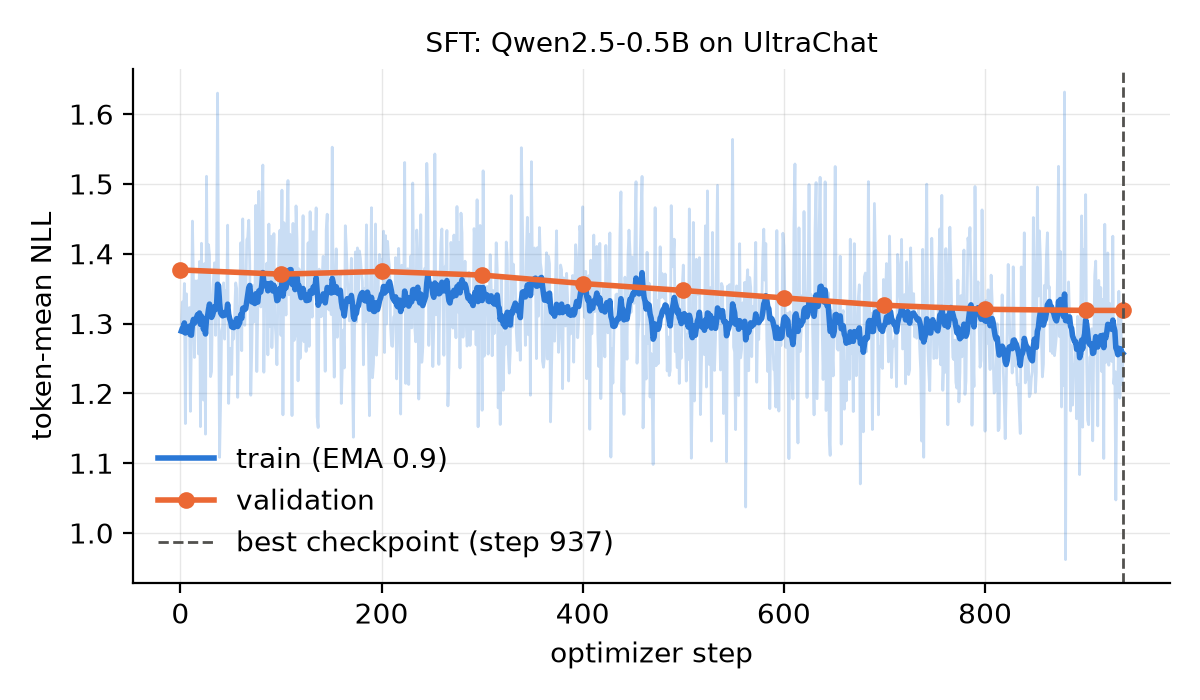
\includegraphics[width=0.55\textwidth]{figures/sft_loss.png}
\caption{SFT training loss (raw and EMA-smoothed, per optimizer step) and validation loss, with the best checkpoint marked.}
\end{figure}

\begin{figure}[H]
\centering
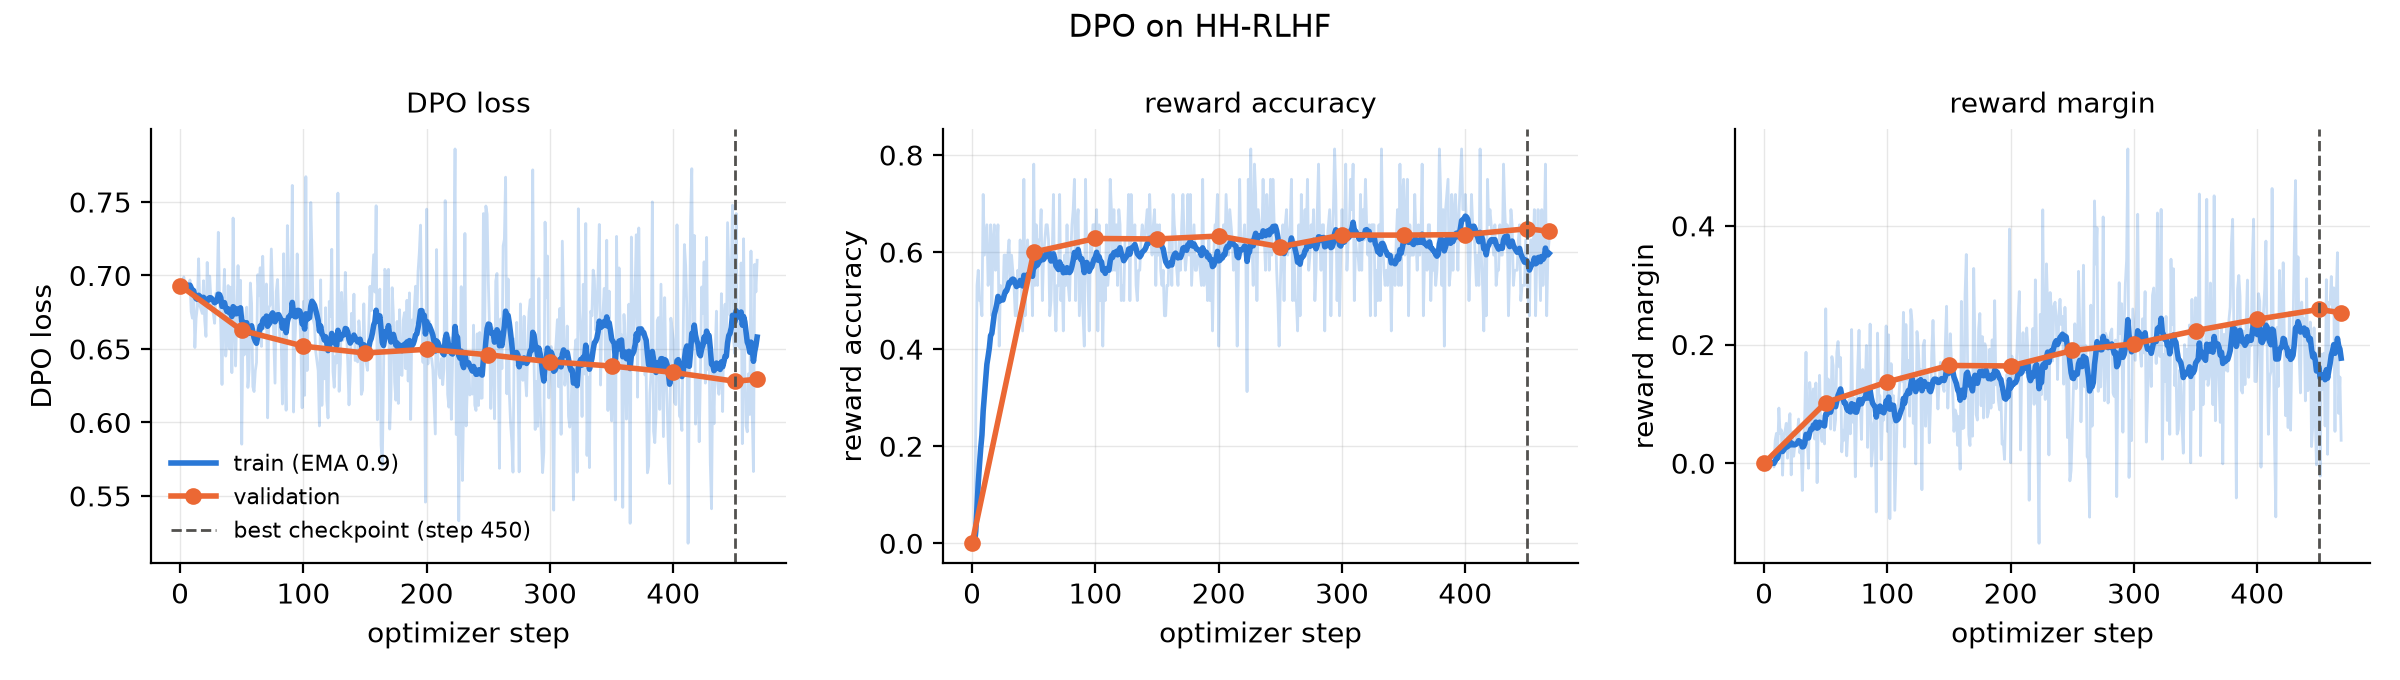
\includegraphics[width=\textwidth]{figures/dpo_hh.png}
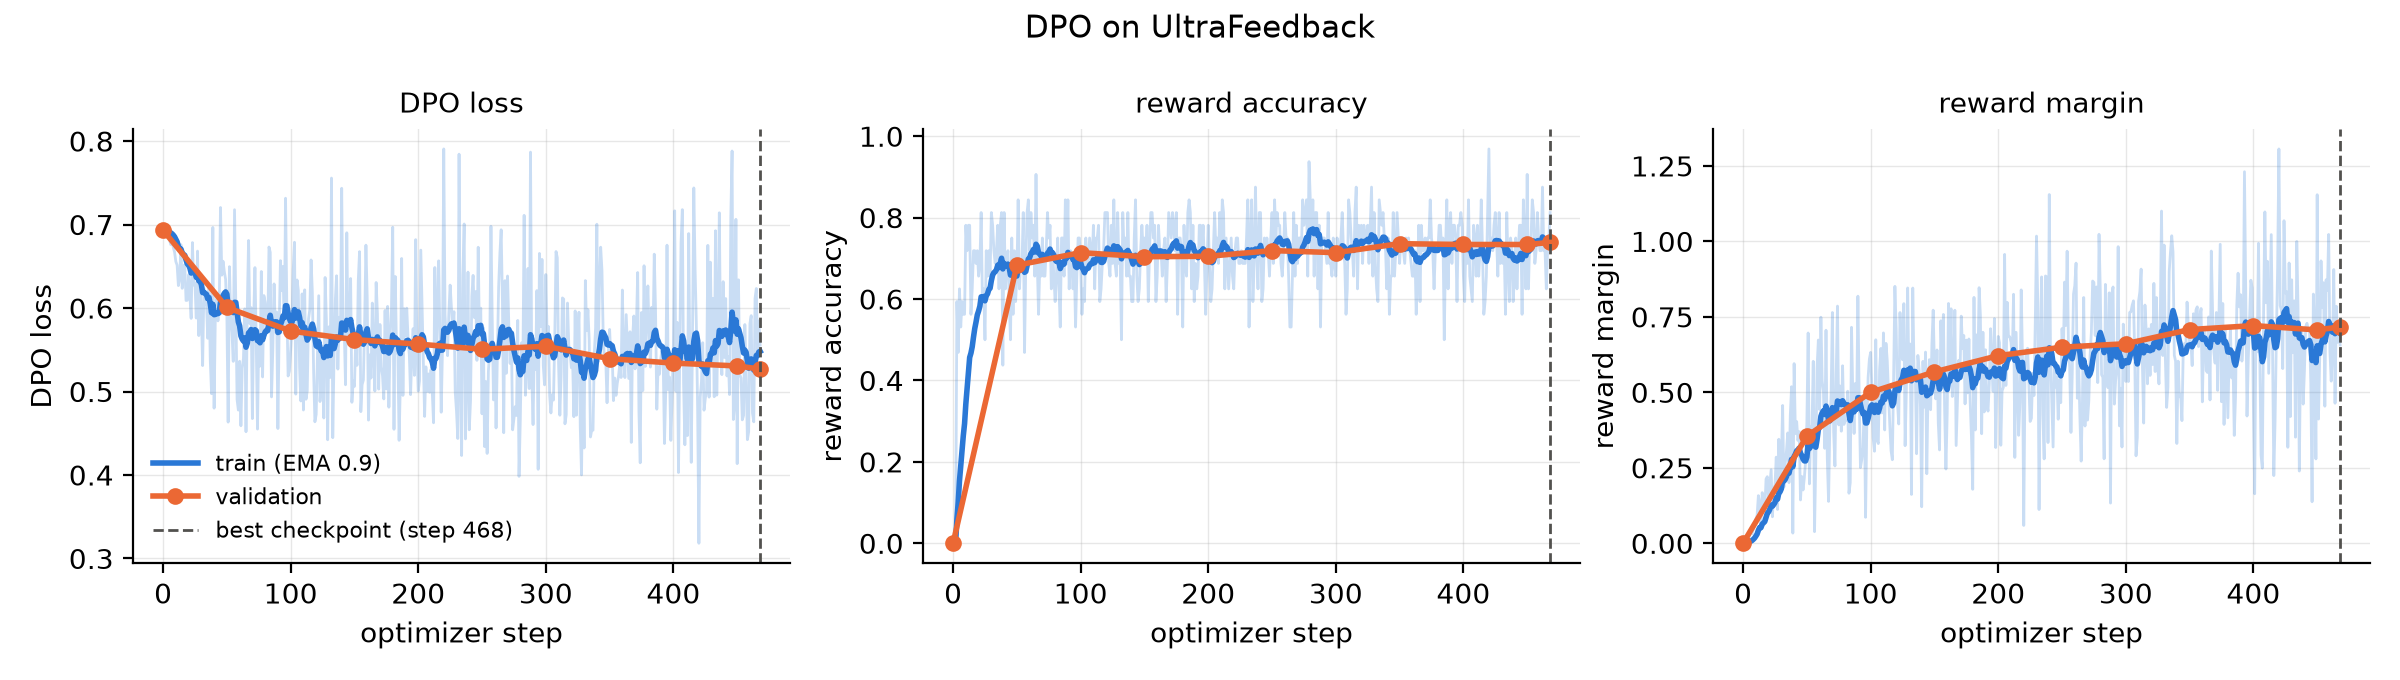
\includegraphics[width=\textwidth]{figures/dpo_ultrafeedback.png}
\caption{DPO loss, reward accuracy and reward margin for both runs. Training curves are EMA smoothed over steps of 32 pairs each, and validation curves use 1{,}000 pairs. In the first step (step 0), the policy is the same as the reference, so the accuracy = 0 and the margin = 0.}
\end{figure}

\textbf{SFT.} The validation loss is nearly constant for the first $\sim$300 steps, then decreases from 1.377 to 1.319 during the cosine decay, and is still slightly decreasing at the last step (937), which is the best checkpoint.
The decline is relatively small since a low loss is already assigned to UltraChat text in the base model.
Generations show that SFT mainly teaches the format: the model answers in the template and gives out EOS to stop.
The median norm of the gradient before clipping was 4.5 and there was no step skipped for fp16 overflow.

\textbf{DPO.} Both runs start exactly at the analytic values: loss $\log 2 = 0.693$, reward accuracy 0 and margin 0, due to the reference being the same as the policy.
\begin{itemize}
\item \textbf{UltraFeedback:} the accuracy of validation reaches 0.68 after 50 steps, and then slowly rises to 0.739, where the margin is at 0.72. The last step (468) is the most suitable checkpoint.
\item \textbf{HH-RLHF:} learning is slower and noisier. The validation accuracy at step 50 is 0.60, and the highest validation accuracy, 0.648 at step 450 (margin 0.26), is the submitted checkpoint.
\end{itemize}
The gap corresponds to label noise. Many HH-RLHF pairs are very similar, and the agreement rate of the annotators in such pairs is also known to be low. UltraFeedback pairs are from a ranked scoring with a more apparent difference in quality.
At the best step in HH-RLHF, both implicit rewards are negative (chosen $-0.35$, rejected $-0.61$): the policy decreases the likelihood of both answers, and decreases the rejected answer further. For the case of UltraFeedback, the chosen reward is still close to zero, and the rejected reward is decreased to $-0.67$.
Gradient-norm clipping at 1.0 was always on, as the sequence log-probabilities are sums over hundreds of tokens, resulting in median pre-clip norms of 42 (HH) and 57 (UF).
During each run, the loss scaler for fp16 mode skipped 3 out of 468 optimizer steps (HH: steps 1, 5, 141; UF: steps 1, 8, 285). The first two skipped steps in each run happened during calibration of the scale.
The validation curves do not appear to be overfitting within one epoch, since there is no validation curve at the end that is rising. Only preference fit (not response quality) is described by these curves; response quality is measured in Section~\ref{sec:results}.

\textbf{LoRA-DPO.} The held-out reward accuracy is 1.0 from the first evaluation (step 5), and the margin increases steadily to 2.15. The 20 pairs that were not used in the training process are easily separated (styled vs.\ neutral), so the accuracy alone is not particularly indicative of the quality of the style transfer.

\begin{figure}[H]
\centering
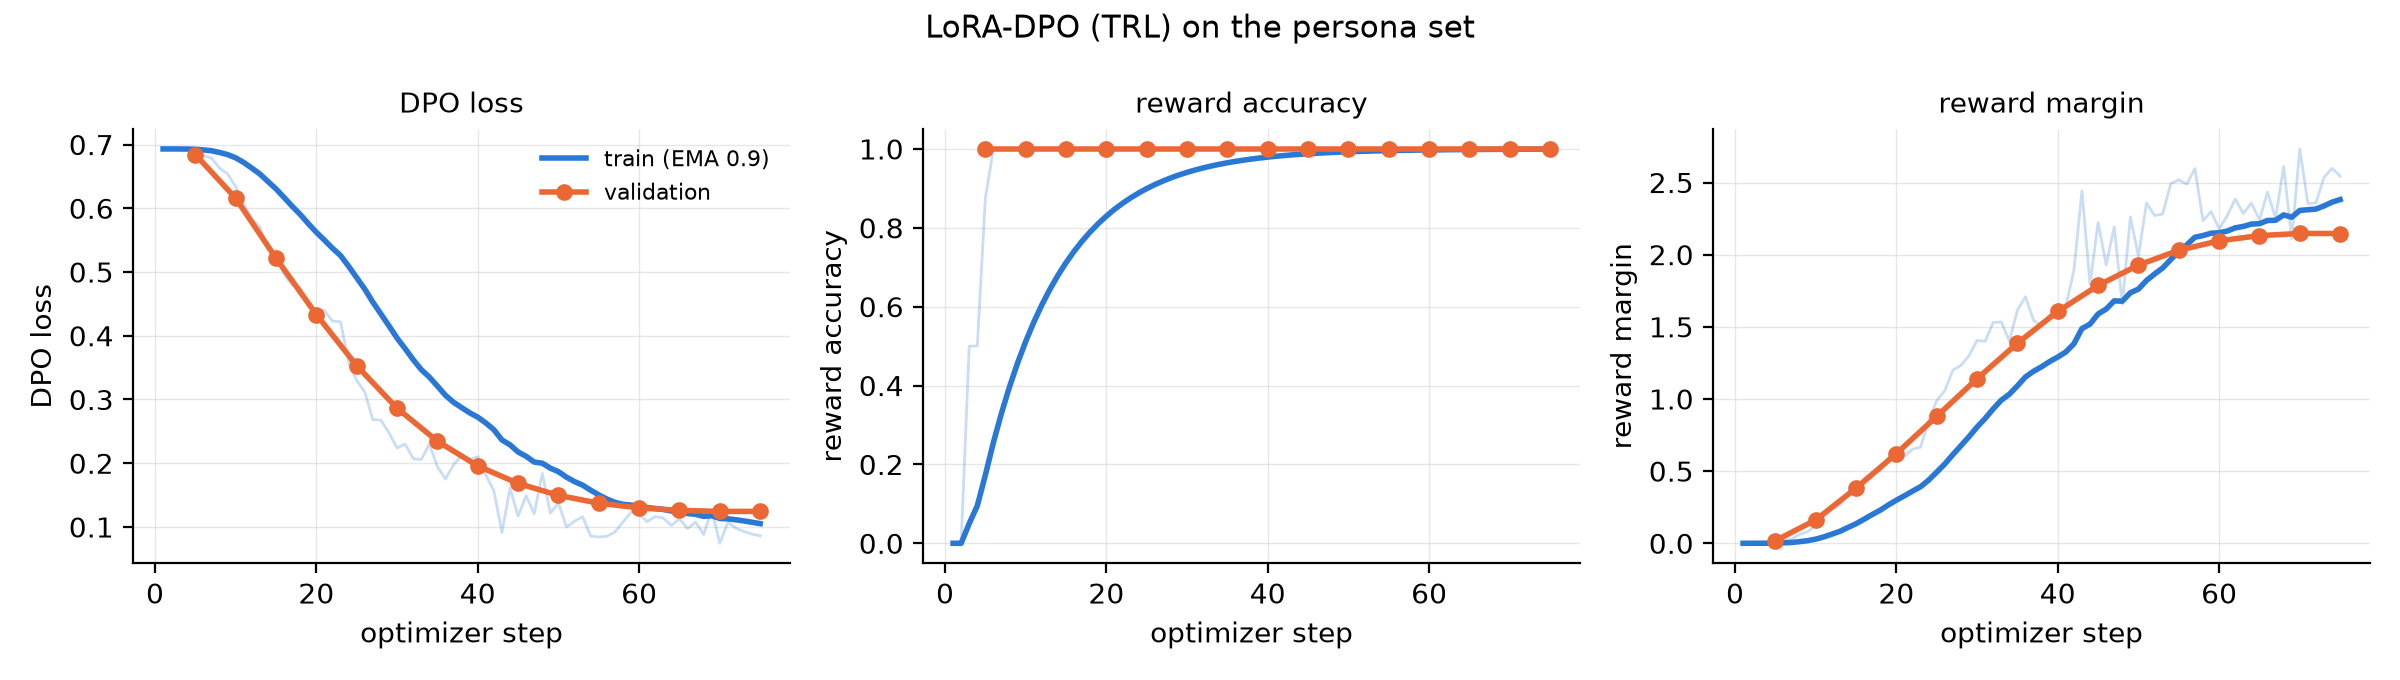
\includegraphics[width=\textwidth]{figures/lora_persona.png}
\caption{LoRA-DPO (TRL) training on the persona set: training loss (logged each step) and held-out metrics on 20 pairs (every 5 steps).}
\end{figure}

\section{DPO versus SFT Results}\label{sec:results}

\begin{itemize}
\item \texttt{google/gemini-3.6-flash} is used as the judge through \texttt{kaggle\_benchmarks}.
\item Groups of 5 pairs per request; requests are at least 5\,s apart and no more than 3 attempts are allowed per group.
\item A/B order randomized per pair (seed 42), and the judge only gets to see ``Response A/B''.
\item There are two ways to calculate win rate: counting ties as half a win and not counting ties.
\end{itemize}
The prompt for the HH set is based on a safety rubric: helpfulness criteria + appropriate refusal, privacy, calibration, safe redirection, penalising over-refusal. The general rubric (helpfulness, correctness, instruction following, conciseness, formatting, no hallucination) is the basis for AlpacaEval.
\begin{itemize}
\item Sometimes, the judge would return a group from the first pass missing one pair. Those groups were retried, and 244 of 979 judged pairs (25\%) needed a second attempt.
\item Those pairs that remained unsolved after 3 attempts were added to \texttt{*\_failures.jsonl}, and a rerun with \texttt{--reuse\_judgments} judged only these pairs.
\item Lastly, 1 pair out of 980 was left unresolved and thus considered a failure (UltraFeedback set).
\item All judgments were parsable (unknown = 0).
\end{itemize}
The 95\% interval is a normal approximation to the win rate (no ties).

\begin{table}[H]
\centering\small
\caption{Pairwise judgments of each DPO model against the SFT baseline on the same prompts with the same decoding (\texttt{outputs/eval/*\_judged\_summary.json}).}
\label{tab:results}
\setlength{\tabcolsep}{4pt}
\begin{tabular}{llrrrrrccc}
\toprule
\textbf{Comparison} & \textbf{Eval set} & $\boldsymbol{n}$ & \textbf{Win} & \textbf{Tie} & \textbf{Loss} & \textbf{Fail} & \textbf{WR (ties $\tfrac{1}{2}$)} & \textbf{WR (no ties)} & \textbf{95\% CI} \\
\midrule
HH-DPO vs SFT & HH eval & 300 & 146 & 20 & 134 & 0 & 0.520 & 0.521 & [0.46, 0.58] \\
UF-DPO vs SFT & AlpacaEval & 300 & 145 & 32 & 122 & 1 & 0.538 & 0.543 & [0.48, 0.60] \\
\midrule
\multicolumn{10}{l}{\emph{Secondary analysis (alignment tax)}} \\
HH-DPO vs SFT & AlpacaEval & 300 & 111 & 68 & 121 & 0 & 0.483 & 0.478 & [0.41, 0.54] \\
\bottomrule
\end{tabular}
\end{table}

\begin{table}[H]
\centering\small
\caption{HH-DPO vs SFT by category (30 prompts each; win -- loss -- tie).}
\label{tab:hhcat}
\begin{tabular}{lccc@{\hspace{2.5em}}lccc}
\toprule
\textbf{HH category} & \textbf{W} & \textbf{L} & \textbf{T} & \textbf{HH category} & \textbf{W} & \textbf{L} & \textbf{T} \\
\midrule
harmful instructions & 18 & 9 & 3 & safe transformation & 15 & 12 & 3 \\
benign helpfulness & 19 & 11 & 0 & cyber abuse & 12 & 14 & 4 \\
legal / financial safety & 18 & 11 & 1 & calibration and uncertainty & 9 & 17 & 4 \\
hate or harassment & 16 & 11 & 3 & privacy and doxxing & 16 & 14 & 0 \\
medical safety & 16 & 12 & 2 & self-harm support & 7 & 23 & 0 \\
\bottomrule
\end{tabular}
\end{table}

\begin{table}[H]
\centering\small
\caption{Response length (\texttt{outputs/eval/analysis.json}, from \texttt{scripts/analyze\_results.py}).}
\label{tab:length}
\begin{tabular}{lccccccc}
\toprule
 & \multicolumn{4}{c}{\textbf{AlpacaEval}} & \multicolumn{3}{c}{\textbf{HH eval}} \\
\cmidrule(lr){2-5}\cmidrule(lr){6-8}
 & Base & SFT & DPO-UF & DPO-HH & Base & SFT & DPO-HH \\
\midrule
Mean response tokens & 410 & 184 & 266 & 162 & 392 & 169 & 142 \\
Hit the 512-token cap & 59\% & 4\% & 7\% & 5\% & 49\% & 2\% & 1\% \\
\bottomrule
\end{tabular}
\end{table}

\textbf{Persona result (LoRA) (reported separately).} The LoRA-DPO model is compared to the unmodified SmolLM2-360M-Instruct on the 40 persona prompts, using two separate judge rubrics.
\begin{itemize}
\item \textbf{Persona style rubric} (faithful to Ramsay style persona; helpful and safe): 19 wins, 8 ties, 13 losses. That is a win rate of 0.575 with ties as half, 95\% CI [0.42, 0.76] without ties.
\begin{itemize}
\item The gains are in cooking (8--1--1) and general help (5--0--5).
\item Coding (3--5--2) and safety-sensitive prompts (3--7--0) lose.
\end{itemize}
\item \textbf{Helpfulness and safety rubric} (safety rubric above): 11 wins, 2 ties, 27 losses. This is a win rate of 0.300, 95\% CI [0.15, 0.43] without ties, with losses in every category.
\end{itemize}
The adapter was thus more ``faithfully'' stylized when it came to the training data (cooking), but less useful. It introduced inaccuracies in its content (e.g.\ it claims the grey, limp green beans were boiled ``not long enough'', whereas the base model correctly claims too long) and used theatrical framing in place of substance.

\section{Interpretation and Error Analysis}

\textbf{Which model is superior and how much.} DPO is very close to SFT (as measured).
\begin{itemize}
\item The clearest improvement is for UltraFeedback DPO, at 54.3\% of decided pairs, with the 95\% interval just crossing 50\%.
\item For safety, HH-RLHF DPO is virtually tied with SFT (52.1\%).
\item On AlpacaEval, HH-DPO is slightly worse than SFT (47.8\%). This is in line with a small alignment tax; however, it is not significant.
\end{itemize}
Where the preference data matches the evaluation, the judge prefers DPO a little more often than not, but this change is much smaller than the change from the base model to SFT, which turned 59\% runaway generations into answers that stop (Table~\ref{tab:length}).

\textbf{Interpretation: UltraFeedback.} The UltraFeedback model writes 45\% longer answers than SFT (266 tokens vs.\ 184 tokens), it has more structure, and it includes more examples and finally a summary at the end. This aligns with UltraFeedback's desire for in-depth responses such as those provided by GPT-4.
The judge was not only looking for length: the longer answer in decided pairs only won 48\% of the time.
The wins are in the content that's more relevant, such as the answer to a career inquiry that listed job titles, and fewer obvious errors made (the judge noticed a colour symbolism in the SFT answer relating to Christmas wreaths that was not there).
The losses result from missing details (paper summary that leaves out a key mechanism). Facts are not improved: both models include a gorilla and living bears as ``extinct bear species''. DPO changes preference, it DOES NOT change knowledge.
While the accuracy of the validation reward is high (0.74), this is only partly visible in judged quality. The policy learned to separate UltraFeedback pairs much more than it learned to generate improved responses.

\textbf{Interpretation: HH-RLHF.} The near-tie is explained by the per-category table (Table~\ref{tab:hhcat}).
\begin{itemize}
\item DPO's strengths: harmful instructions (18--9), legal/financial safety (18--11), benign helpfulness (19--11).
\item It is down on both self-harm support (7--23) and calibration (9--17).
\item This is evident in the outputs: HH-DPO reproduces the assistant voice of HH-RLHF, such as the disclaimer ``I am not capable of feeling emotions, but\ldots'', lowercase beginning of sentences, and also shorter answers (142 vs.\ 169 tokens). When asked to write a supportive message for someone who thinks they are a burden, its answer was called ``robotic'' by the judge, who preferred SFT's heartfelt message template.
\item A lot of ``wins'' for DPO are only ``less bad'' if the request is bad. Both models yield steps for car sabotage; the DPO answer starts to go towards diagnosing the car, and the judge tallied this as a safe reframe.
\item These two models can't be guaranteed to refuse. The percentage of explicit refusal phrases is 2\% (SFT) and 5\% (DPO).
\end{itemize}
These patterns are consistent with the training diagnostics. The HH validation accuracy stopped improving at 0.65, as would be expected given the known label noise in HH-RLHF, and both implicit rewards were negative, which means DPO also reduced the probability of the selected responses. The policy shifted more in style (tone, disclaimers, length) than in safety behaviour with 0.5B parameters and $\beta = 0.1$ after one epoch.

\textbf{Interpretation: persona LoRA.} Style alignment worked where the data was: cooking prompts got a strong Ramsay voice. It didn't generalise to coding and safety prompts, where the insults hurt. The typical trade-off is reflected in the large loss on helpfulness and safety (30\% win rate).
The persona pairings consist of a stylized but correct selected response and a neutral and correct rejected one, which is typically de-emphasized by the DPO. Three epochs of a 360M model with a learning rate of $5\times10^{-5}$ created disturbance in the content as well. This was completely masked by the held-out reward accuracy of 1.0.

\textbf{Takeaways.} Reward accuracy and DPO loss measure fit to preference pairs, not answer quality. Both DPO tracks were more of a change in style than in substance, and the safety track shows that data collected from preferences can be used to learn disclaimers (unwanted surface behavior) as well as the desired behavior.

\section{Limitations and Reproducibility}
\begin{itemize}
\item \textbf{Judge bias and noise.}
  \begin{itemize}
  \item One LLM judge (one judgement per pair).
  \item Among decided pairs, the response in position A won 55--60\% of the time. The ordering is random (151 of 300 DPO responses are in position A), so there is noise but no bias in favor of either model.
  \item There are some examples of judgment reasons that are false, like in the above car-sabotage case.
  \item If the pairs could be judged both ways, position bias would be lessened.
  \end{itemize}
\item \textbf{Small evaluation sets and 1 seed.}
  \begin{itemize}
  \item The interval on the win rate around 300 prompts is $\pm$6\%, which means that none of the three differences in win rate between DPO and SFT is significant at the 5\% level. There are 40 prompts in the persona set.
  \item There are some duplicate instructions in the HH evaluation set provided.
  \item The same seed (42) is used for all runs.
  \end{itemize}
\item \textbf{Compute.}
  \begin{itemize}
  \item We did not sweep $\beta$ and learning rate on T4s; each DPO run was one epoch with a fixed $\beta = 0.1$.
  \item About 28\% of the selected responses were truncated at 512 tokens for UltraFeedback, measured on a sample of 2{,}000 pairs.
  \end{itemize}
\item \textbf{Reproducibility.}
  \begin{itemize}
  \item The configuration, data summary and per-step metrics of each run are in \texttt{outputs/<run>/}.
  \item The \texttt{outputs/generations/} folder contains the generations. Pairwise files, judgments, failures and summaries are in \texttt{outputs/eval/}.
  \item \texttt{scripts/plot\_metrics.py} generates the figures and \texttt{scripts/analyze\_results.py} provides data on length and judge-bias.
  \item Each stage of these experiments is executed sequentially in the Kaggle notebooks \texttt{notebooks/01} -- \texttt{notebooks/06}.
  \end{itemize}
\end{itemize}

\begin{thebibliography}{9}\small
\bibitem{dpo} R.~Rafailov et al. Direct Preference Optimization: Your Language Model is Secretly a Reward Model. NeurIPS 2023.
\bibitem{qwen} Qwen Team. Qwen2.5 Technical Report. 2024.
\bibitem{ultrachat} N.~Ding et al. Enhancing Chat Language Models by Scaling High-quality Instructional Conversations. 2023.
\bibitem{hh} Y.~Bai et al. Training a Helpful and Harmless Assistant with Reinforcement Learning from Human Feedback. 2022.
\bibitem{uf} G.~Cui et al. UltraFeedback: Boosting Language Models with High-quality Feedback. 2023.
\bibitem{alpacaeval} X.~Li et al. AlpacaEval: An Automatic Evaluator of Instruction-following Models. 2023.
\bibitem{lora} E.~Hu et al. LoRA: Low-Rank Adaptation of Large Language Models. ICLR 2022.
\end{thebibliography}

\end{document}
